\documentclass[conference]{IEEEtran}
%	\IEEEoverridecommandlockouts
\usepackage{cite}
\usepackage{amsmath,amssymb,amsfonts}
%	\usepackage{algorithmic}
\usepackage[dvipdfmx]{graphicx}
\usepackage{graphicx}
\usepackage{color}
\usepackage{textcomp}
\usepackage{xcolor}
\definecolor{blue}{rgb}{0.00, 0.00, 1.00}
\usepackage{listings}
\usepackage{datetime2}
\usepackage{algorithm}
\usepackage{algorithmicx}
\usepackage{algpseudocode}
\def\BibTeX{{\rm B\kern-.05em{\sc i\kern-.025em b}\kern-.08em T\kern-.1667em\lower.7ex\hbox{E}\kern-.125emX}}
\lstset{
  language={Fortran},
  basicstyle={\ttfamily},
  identifierstyle={\small},
  %	commentstyle={\smallitshape},
  % keywordstyle={\small\bfseries},
  keywordstyle={\small},
  ndkeywordstyle={\small},
  %	stringstyle={\small\ttfamily},
  frame={tb},
  breaklines=true,
  columns=[l]{fullflexible},
  numbers=left,
  xrightmargin=0zw,
  xleftmargin=2zw,
  numberstyle={\scriptsize},
  stepnumber=1,
  numbersep=1zw,
  lineskip=-0.5ex,
  %	belowcaptionskip=10pt,abovecaptionskip=10pt
}


\begin{document}

\title{
\textcolor{blue}{as of \DTMnow} \\
Performance evaluation and visualization of scientific applications using PMlib
}

\author{
\IEEEauthorblockN{1\textsuperscript{st} Kazunori Mikami}
\IEEEauthorblockA{\textit{Flagship 2020 Project} \\
\textit{Riken R-CCS}\\
Kobe, Japan \\
kazunori.mikami@riken.jp}
\and
\IEEEauthorblockN{2\textsuperscript{nd} Kenji Ono}
\IEEEauthorblockA{\textit{RIIT} \\
\textit{Kyushu University}\\
Fukuoka, Japan \\
keno@cc.kyushu-u.ac.jp}
}

\maketitle

\begin{abstract}
Sustained computational performance of scientific applications on HPC systems
is often observed much lower than the maximum system performance.
Understanding this gap requires multi-perspective analysis, i.e., the system
architecture perspective to evaluate the characteristics of micro architecture
elements such as processor core and memory, and the applications perspective
to correlate the theoretical computation coded as the source program with the
computation workload produced by compilers.
The authors developed PMlib open source library to address such synthetic analysis.
PMlib provides the way to report the arithmetic workload counted manually from
the source code, as well as the actually executed system workload.
It also provides the detail utilization report of processor specific hardware
including the categorized SIMD instruction statistics, the layered cache
hit/miss rate, and the corresponding bandwidth up to memory,
which are captured via hardware performance counters (HWPC).
Using PMlib, users can conduct synthetic analysis of the application
performance, and obtain the hint for further optimized execution of
the applications.
\end{abstract}

\begin{IEEEkeywords}
performance evaluation,
arithmetic workload,
system workload,
performance visualization,
open source library,
PMlib
\end{IEEEkeywords}

\section{Introduction}
In the development and the productive phase of the scientific application,
the performance evaluation is frequently conducted on the target HPC systems.
in order to understand the performance characteristics
of the application on the target system, and to explore the possibility of
applying further optimization to the software for elapsed time reduction.
As a background of this,
depending on the type of application and HPC system,
we frequently observe the situation where
the sustained computational performance of scientific applications on HPC
systems is much lower than the theoretical maximum performance
expected from the system specification,

Prededing studies to account for this gap between the achieved
performance and the maximum performance addressed mostly from architecture
point of view,
some mentioning the utilization of parallel functional units,
some mentioning the locality of data residing on memory/cache hiererchy.

The performance is measured in the unit of conducted workload / elapsed time.
We should remind that the definition of workload measurement can vary,
usually chosen from one of the the followings,
the arithmetic workload defined by the applications in their source program,
and the system workload actually executed on HPC systems that is represented
as machine instructions which is measured with hardware performance counters
(HWPC).
The difference in the performance based on these two workload definitions
can be significant as explained in section \ref{workload-evaluation},
and is sometimes confusing to application users.
%	Obvious relational effect of job manager and the system workload is not
%	the focus of this paper.

PMlib, an open source library for performance evaluation,
\cite{PMlib:webpage-public}
has the functionality
to explicitly measure the arithmetic workload counted in the source program
using manually formulated argument, as well as the functionality
to automatically measure the HWPC event base workload,
thus providing users an option to compare the difference in workloads.

In measuring the HWPC events, PMlib utilizes PAPI \cite{PAPI:5.6} low level API.
PMlib has its own scheme to choose the related HWPC event sets and to sort out
the event statistics according to run time environment variables, making it
easier to extract the statistics of interest.
Choosing the correct set of events for specific processor type and
translating the accumulated counts into meaningful performance index can be
non-trivial work if without PMlib.
The output information from PMlib is a blocked text report based on
the time averaged performance statistics, by default.
It also produces the Open Trace Format
\cite{Knupfer:2006}, \cite{OTF:webpage-public}
tracing file reflecting
the shorter interval statistics which can be read by Web browser
visualization tool TRAiL.% \cite{}.

In this paper, the difference between the arithmetic workload and the system
workload is clarified.
Next, the PMlib's useful feature for performance evaluation is shown.
Finally, some examples of the performance evaluation using PMlib
are shown indicating the merit obtained from multi-perspective analysis.

\section{Computational workload and Performance evaluation}
\label{workload-evaluation}

\subsection{user perspective}
\label{subsection:user-perspective}

The term "computational workload" for scientific application developpers
is generally perceived as the total volume of arithmetic operations,
expressed by the formulas in the source code written in Fortran/C/C++.

The workload at this level can be simply represented as below:
%	\begin{align}
%	\end{align}
\begin{equation}\label{eq:arithmetic-workload}
	Workload = \sum_{i=1}^{types} W_{ops}(i)
\end{equation}
where $ W_{ops}(i) $ is the number of operations for the
corresponding arithmetic type such as
1:add, 2:sub, 3:mult, 4:div, 5:max, 6:min, 7:sqrt, etc.

In the development phase of the HPC applications, practical developers
choose and deploy the numerical algorithm which require the least
amount of arithmetic operations through the scientific consideration,
aiming to reduce the elapsed time to obtain the desired simulation results.
The workload in this context is named arithmetic workload in this paper.

The formulas in the source code are then compiled to corresponding assembly
instructions.
Each arithmetic statement is mapped to a sequence of multiple instructions.
We use "weight factor" to map the original arithmetic operations to the
generated instructions to quantify the relationship.
Assuming a simple weight factor $ c $ for each type of
arithmetic operations, 
the workload at this point can be represented as below:
\begin{equation}\label{eq:application-workload}
		Workload = \sum_{i=1}^{types} \left(c(i)\times W_{ops}(i)\right)
\end{equation}
% workload_{system}

This workload formula is named application workload in this paper.
The application workload formula is a simple representation of the original
arithmetic and provides easy-to-understand relationship between the change
in the algorithm and the resulting change in the workload.

The application performance is evaluated based on the elapsed time as below.
\begin{align}\label{eq:performance-workload-time}
Performance = Workload / Time 
\end{align}

For example, Linpack (HPCC) 
\cite{}
workload is calculated based on the arithmetic workload formula
using the addition and multiplication terms.
\begin{align}
		Workload & = W_{ops}(add) + W_{ops}(mult) \\
		W_{ops}(add) & = W_{ops}(mult) = 1/3 N^{3} + 3/4 N^{2}
\end{align}
where N is the size of the matrix to be solved.
The linpack performance value "flops" is reported using this workload as
\begin{align*}
Gflops = N^{2} \times ( 2/3 * N + 3/2 ) \times 1.0^{-9} / Time 
\end{align*}
In linpack example, the application performance is based on
the same weight factor $ c = 1.0 $ 
for both addition and multiplication, which is actually reflecting the
arithmetic workload and performance.

The workload formulation in the form of
\eqref{arithmetic-workload}
or
\eqref{application-workload}
provides the general idea of the theoretical workload requirement by the
application.
PMlib can be used to formulate these arithmetic and application workload
as explained in section \ref{section:PMlib}.

\subsection{system perspective}
\label{subsection:system-perspective}

For large size applications, it can be difficult to formulate
the arithmetic workload or the application workload.
Even if the arithmetic workload formulation is accompplished,
the mapping of weight factor can be complex.

Mapping mathematical functions to the native instructions
depends not only on the systems architecture but also on the compiling
software and its optimization options.
There are multiple choices of available instructions for the same
arithmetic operation on modern processors.
The choice of instructions from scalar/vector syntax is made by
compiler optimization strategy, for example.
In vector, the degree of parallelism, i.e. width of simultaneous data
operation, with the effect of loop length is influential.
In scalar, data locality is influential.
Run time hardware behavior including out-of-order execution can not
be reflected to static weight factor.
A simple instruction latency and throughput model may not account.

Now we look at the workload and performance from system perspective.
The micro architecture elements including the number of compute cores
in the processor, the degree of parallelism inside each core,
the depth of cache/memory hierarchy and the data move rate at each hierarchy
all have relational impact to how the machine instructions are executed,
thus leading to sustained computing performance.

The fact that the actual numerical computation is accomplished by the
limited set of hardware components, and that the HWPC is available
on modern HPC systems, makes it more practical to obtain the HWPC statistics
and to analyze them for performance evaluation.
Through appropriate APIs, HWPC statistics can be accessed, so does PMlib.

PMlib utilize PAPI \cite{papi-1} low level API to accomplish this,
and calculate the computing workload from the executed instructions.
It provides the processor specific hardware utilization report
including categorized SIMD instruction statistics,
layered cache hit/miss rate, and the corresponding bandwidth upto memory.
It utilizes PAPI low level API for obtaining HWPC event statistics.

PAPI has its own event mnemonics for each type of HWPC proccessors.
For example, floating point operations on
Intel Xeon Skylake Gold processor % no citation \cite{skylake-1} 
are measured as the following events.

%	\begin{lstlisting}[caption={Intel Xeon Skylake f.p. SIMD operations}]
%	\end{lstlisting}
\begin{quote}
\begin{small}
\begin{verbatim}
fpsp1  : "FP_ARITH:SCALAR_SINGLE";
fpsp4  : "FP_ARITH:128B_PACKED_SINGLE";
fpsp8  : "FP_ARITH:256B_PACKED_SINGLE";
fpsp16 : "FP_ARITH:512B_PACKED_SINGLE";
fpdp1  : "FP_ARITH:SCALAR_DOUBLE";
fpdp2  : "FP_ARITH:128B_PACKED_DOUBLE";
fpdp4  : "FP_ARITH:256B_PACKED_DOUBLE";
fpdp8  : "FP_ARITH:512B_PACKED_DOUBLE";
\end{verbatim}
\end{small}
\end{quote}

The sum of these operations multiplied by the corresponding width
of the SIMD instruction, i.e. the weight factor $ c $, gives the
floating point operation workload including single precision
and double precision data types.
%	\begin{multline}
%	W_{hwpc} = fpsp1 + fpdp1 \\
%		+ 4.0*fpsp4 + 8.0*fpsp8 + 16.0*fpsp16 \\
%		+ 2.0*fpdp2 + 4.0*fpdp4 + 8.0*fpdp8;
%	\end{multline}
\begin{align}
	W_{hwpc} & = fpsp1 + fpdp1 \nonumber \\
			& + 4.0*fpsp4 + 8.0*fpsp8 + 16.0*fpsp16 \nonumber \\
			& + 2.0*fpdp2 + 4.0*fpdp4 + 8.0*fpdp8;
\end{align}

The floating point operations on Fujitsu FX100 processor, as second example,
are measured as the following events.
\begin{quote}
\begin{small}
\begin{verbatim}
fpdp1  : "1FLOPS_INSTRUCTIONS";
fpdp2  : "2FLOPS_INSTRUCTIONS";
fpdp4  : "4FLOPS_INSTRUCTIONS";
fpdp8  : "8FLOPS_INSTRUCTIONS";
fpdp16 : "16FLOPS_INSTRUCTIONS";
\end{verbatim}
\end{small}
\end{quote}
The floating point operation workload including single precision
and double precision data types is given as:
\begin{align}
	W_{hwpc} & = fpdp1 + 2.0*fpdp2 + 4.0*fpdp4 \nonumber \\
			& + 8.0*fpdp8 + 16.0*fpdp16; 
\end{align}

We call the workload measured in this fashion as HWPC workload,
and the evaluated performance as HWPC performance.
HWPC performance is commonly used in the HPC systems evaluation.


\subsection{difference in workloads}
\label{subsection:difference-in-workloads}

We now look at an example of situations where the quantitative difference of
the user perspective arithmetic workload and
the system perspective HWPC workload is significant.
Fig.\ref{fig:workload-user} and fig.\ref{fig:workload-system} show
the workload defined in above two context. The Y-axis shows the
corresponding performance given by \eqref{eq:performance-workload-time}.
The difference ranges from 1.0 to 18.0 depending on the type of
arithmetic, and stays mostly constant over various loop length.
In order to obtain these results, PMlib user mode report and PMlib HWPC mode
report were used.
This particular example actually represents the
difference between the arithmetic workload and the application workload,
and the major reason comes from the number of instructions needed to
compute square root and division.
%	\begin{figure}[tb]
%	\centering
%	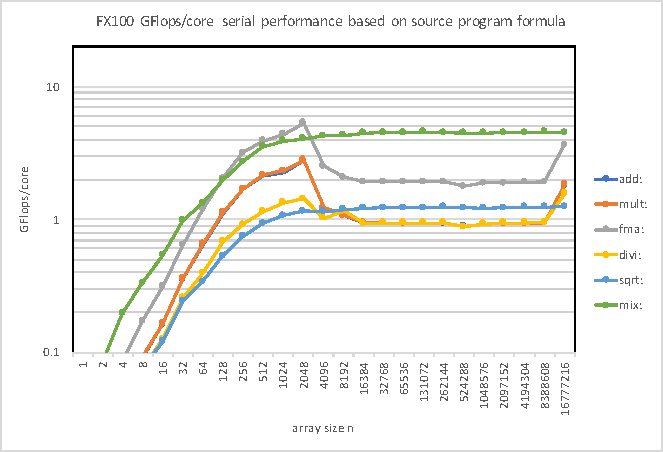
\includegraphics[width=0.45\textwidth]{figs/workload-user.pdf}
%	\caption{workload-user}
%	\label{fig:workload-user}
%	\end{figure}
\begin{figure}[tb]
\begin{minipage}{0.49\hsize}
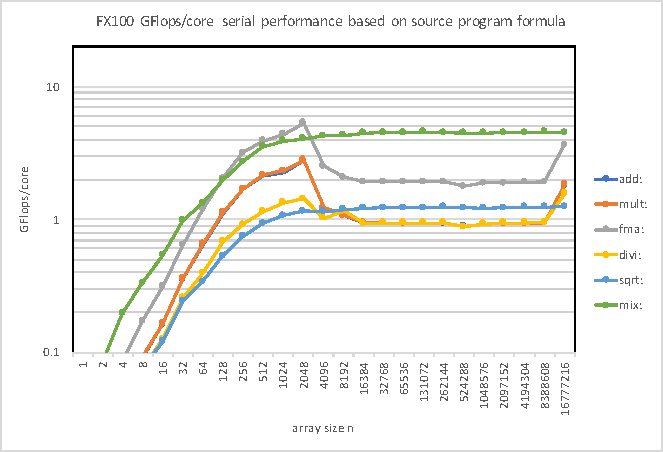
\includegraphics[width=\textwidth]{figs/workload-user.pdf}
\caption{workload-user}
\label{fig:workload-user}
\end{minipage}
\begin{minipage}{0.49\hsize}
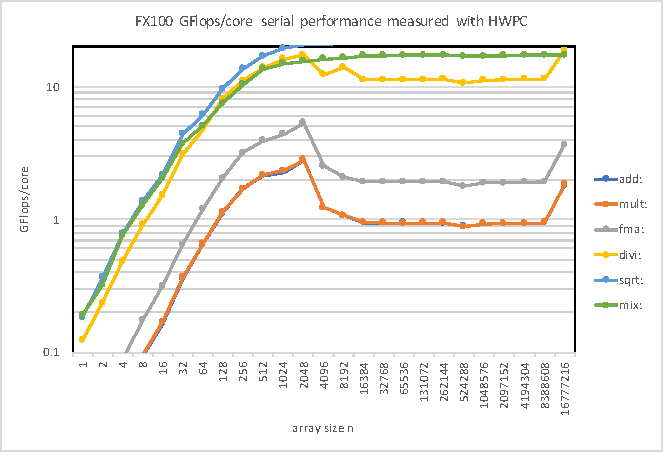
\includegraphics[width=\textwidth]{figs/workload-system.pdf}
\caption{workload-system}
\label{fig:workload-system}
\end{minipage}
\end{figure}
This simple example indicates that the performance evaluation of
scientific applications on HPC systems must be associated with the clear
difinition of workload, and that, if conditions allows, evaluation should be
conducted both in user perspective and in system perspective.

\section{PMlib}
\label{section:PMlib}

\subsection {about PMlib}

PMlib is an open source library to monitor the scientific applications
performance. 
\cite{PMlib:webpage-public},

PMlib is able to measure the listed types of workload discussed in the previous
section, i.e. arithmetic, application and HWPC workload.
Users insert the PMlib start/stop API statements in the source code.
Each measuring section has minimal properties such as name, type of operation,
exclusiveness, and the workload value.
The report from PMlib is classified into threads, processes, sections,
depending on the controlling environment variable.

\subsection{PMlib API}
\label{subsection:PMlib-API}

PMlib APIs can be called from C++ and Fortran programs.
There are only a handful APIs which must be called in most applications.
C++ APIs are shown in table \ref{tab:PMlib-API}. There are equivalent
Fortran APIs who are named as $ f\_pm\_{C++API} $.

\begin{table}[tb]
\scriptsize
\caption{list of PMlib basic APIs}
\label{tab:PMlib-API}
\footnotesize
\begin{tabular}{l|l|l} \hline
\scriptsize
C++	& function	&	arguments	\\ \hline
\hline
initialize	& initial setup	& number of sections (optional)	\\ \hline
setProperties	& set sections property	& label, type, exclusiveness \\ \hline
start	& start of section	& label \\ \hline
stop	& end of section	& label, arithmetic workload (optional)	\\ \hline
print	& basic report	& filename, comments, sort order	\\ \hline
\hline
printDetail	& per process report	& filename, sort order	\\ \hline
printThreads	& per thread report	& filename, sort order	\\ \hline
\end{tabular}
\end{table}

A Fortran program calling PMlib will look like as below.

%	\begin{lstlisting}[caption={using PMlib in Fortran program}]
\begin{lstlisting}
program main
call f_pm_initialize (Nsections)
call f_pm_setproperties ("section1",icalc,iexcl)
call f_pm_start ("section1")
call some_computation (fops)
call f_pm_stop ("section1",fops,ncall)
call f_pm_print ("",isort)
call f_pm_printdetail ("",ilegend,isort)
end
\end{lstlisting}


\subsection {choosing workload type}
PMlib API pair start/stop accumulates the volume of workload internally
towards its report.

The choice of arithmetic workload or HWPC workload is made by a
run time environment variable HWPC\_CHOOSER.
Possible choice of HWPC\_CHOOSER value is:
\begin{quote}
\begin{small}
%	\begin{verbatim}
FLOPS\textbar BANDWIDTH\textbar VECTOR\textbar CACHE\textbar CYCLE%
\textbar user
%	\end{verbatim}
\end{small}
\end{quote}

If the arithmetic workload is measured,
PMlib API accepts the argument holding the value or the formula
of the workload contained inside the section sandwiched by start/stop.
The number of arithmetic operations or the formula must be explicitly
provided by users. Counting up the operation in source can be a tedious job.
If the application is written in Fortran program,
we can take advantage of the related research by Hashimoto
\cite{Hoshimoto:2015}, \cite{ccaebt:HPCAsia2018}
to let the parser program analyze the arithmetic operations
included in Fortran source blocks and produce JSON intermediate report.
Then, a second filter can be used to produce the
Fortran source program including PMlib API calls with
provisioned argument for PMlib.
Fig.\ref{fig:ccaebt4PMlib} shows the schematic flow to accomplish this flow.
\begin{figure}[tb]
\centering
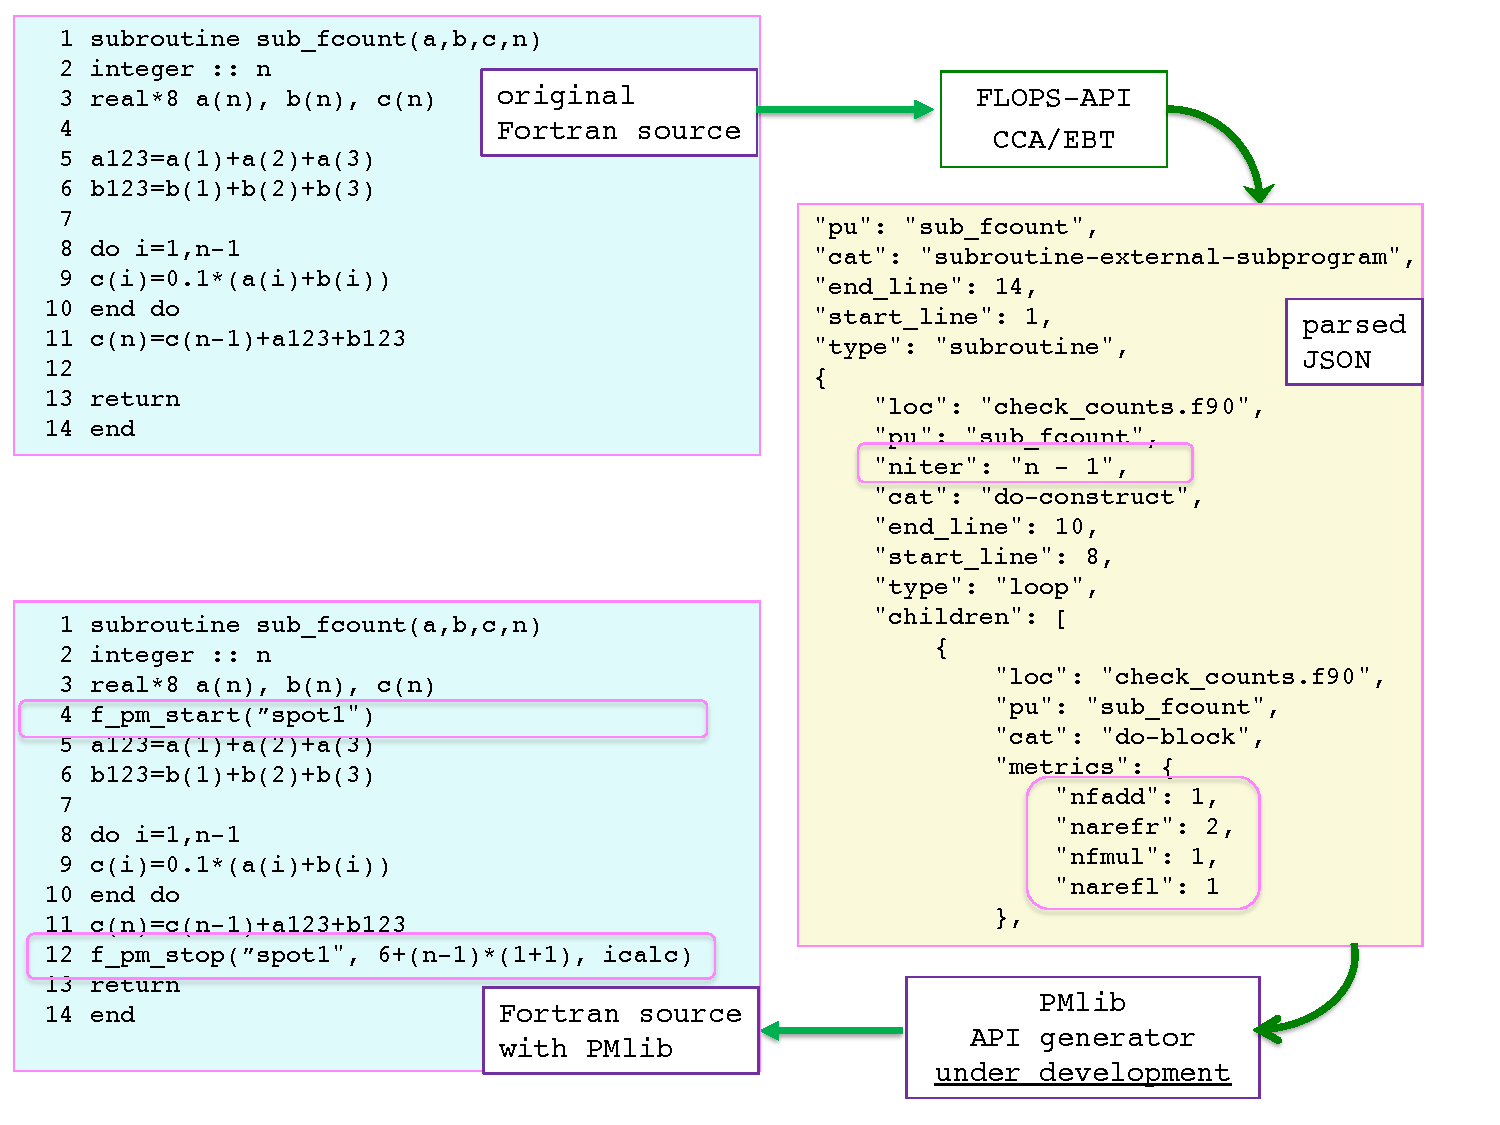
\includegraphics[width=0.45\textwidth]{figs/ccaebt4PMlib.pdf}
\caption{counting the operation with ccaebt}
\label{fig:ccaebt4PMlib}
\end{figure}

If HWPC workload is measured,
PMlib automatically detects the type of hardware, and reads the HWPC
event statistics at each of start/stop API.
In HWPC workload mode, PMlib does not use the user given argument value,
if any.
While PAPI has a good set of user APIs and is well documented,
it is not a simple task to choose the correct native event sets and masks
of the specific target processor instructions and to sort out the event
values for a desired performance category using a limited set of HWPC.
For example,
the standard output from papi\_native\_avail command on a server with
Intel Skylake Gold processor produces 5000+ lines.

PMlib takes the role to interface the application developer's intent to
categorize the performance with the raw information from HWPC, and to
help evaluate the performance.
Once PMlib APIs are coded in the application, PMlib preserves the HWPC
portability. That is, PMlib chooses and reads the appropriate HWPC event
set, if the application is run on different HPC systems.

%	PMlib report example 1
%	PMlib report example 2
%	PMlib report example 3

\subsection{high resolution timer available to PMlib}
PMlib is a portable package, and utilizes linux standard timer
gettimeofday by default. It also has the installation option to utilize
a system specific high resolution low overhead timer if such timer is
available on the platform.

Fig.\ref{fig:precise-timer} shows the comparison of standard timer and
high resolution timer on the two HPC systems in the previous section.
PMlib has provision to use them as installation option.
\begin{figure}[tb]
\centering
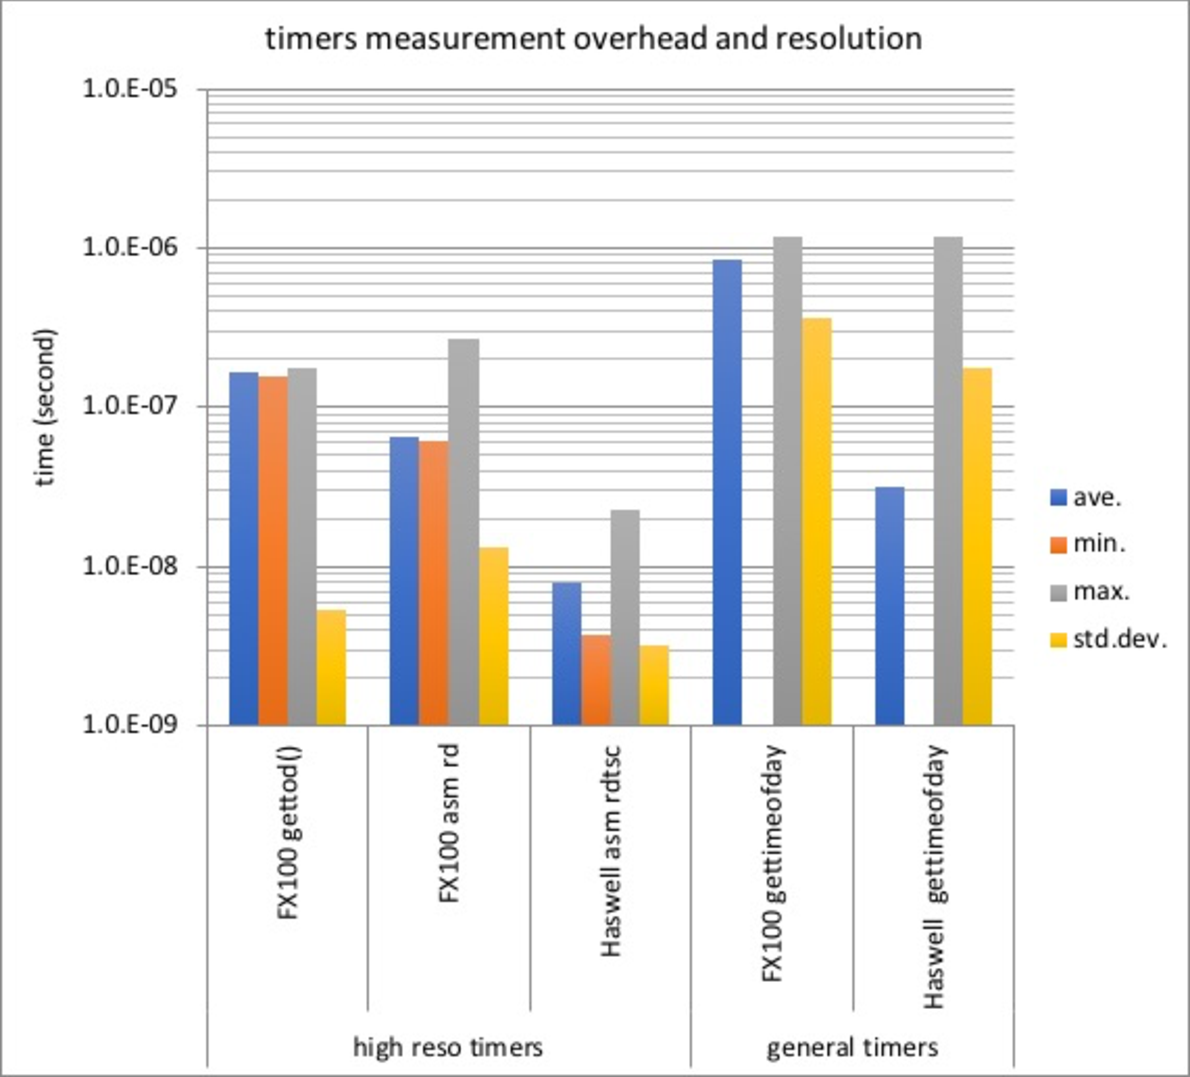
\includegraphics[width=0.45\textwidth]{figs/precise-timer.pdf}
\caption{precise timer v.s. general timer}
\label{fig:precise-timer}
\end{figure}

\subsection{PMlib output information}
\label{subsection:PMlib-output-information}

The output information from PMlib is a blocked text report based on
the time averaged performance statistics, by default.
It also produces the Open Trace Format tracing file reflecting
the shorter interval statistics which can be read by Web browser
visualization tool TRAiL.
\begin{figure}[tb]
\centering
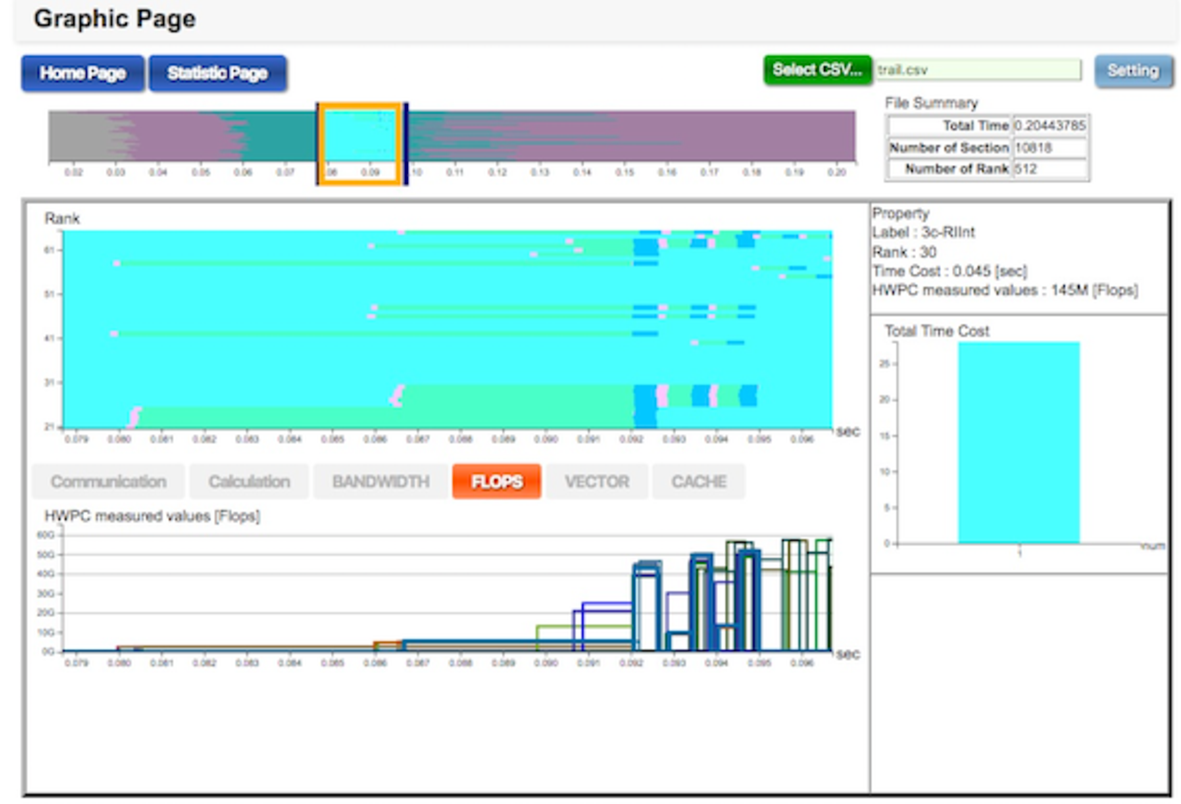
\includegraphics[width=0.45\textwidth]{figs/TRAiL-small.pdf}
\caption{tracing visualization using PMlib and TRAiL}
\label{fig:TRAiL}
\end{figure}

\subsection{other performance evaluation tools and related research}
\label{subsection:related-research}
There has been various tools developed for HPC system  performance evaluation.
In the open source category:
\begin{itemize}
	\item Scalasca \cite{Scalasca:2017},\cite{Scalasca:2010}
			: trace generation, Score-P infrastructure
	\item Extrae \cite{Extrae:webpage} :  trace generation
	\item PAPI \cite{PAPI:5.6} : API to access HWPC
	\item Linux perf tools : API to access HWPC
\end{itemize}
The open source tools are designed to be portable. The functionality of the
tools are distinct, and multiple tools are used in sequence to obtain
the desired performance information.

In the vendor supplied X86 category:
\begin{itemize}
		\item Intel VTune \cite{Intel:VTune}, PGI Profiler \cite{PGI:Profiler}
\end{itemize}

HPC systems also have the performance evaluation tools provided by the
system vendors.
Each of the tools has its own cons and pros.
The system vendor provided tools are integrated and qualified in general,
but is available on the vendor's HPC systems only.

These existing tools all utilize the processor performance information
based on HWPC workload, i.e. system workload.
PMlib appears to be the only tool that enables arithmetic workload evaluation.


\section{performance evaluation using PMlib}
\label{section:using-PMlib}

Some examples of using PMlib for performance evaluation are shown in this
section.
The servers used for the measurements and their processor specifications
are listed in table \ref{tab:server-config}.
\begin{itemize}
{
%	\setlength{\itemsep}{-5pt}
%	\setlength{\topsep}{2mm}
\item SGI Intel Ivybridge server
\item SGI Intel Skylake server
\item Fujitsu prime HPC FX100
}
\end{itemize}

\newif\ifTwoservers
\newif\ifThreeservers
\Twoserversfalse
\Threeserverstrue
%\tiny
%\footnotesize
%\small
\begin{table}[tb]
\scriptsize
\caption{server configuration and maximum performance}
\label{tab:server-config}
\footnotesize

\ifTwoservers
\begin{tabular}{l|c|c} \hline
\scriptsize
system			&	FX100	&	Skylake	\\ \hline
CPU				&	SPARC64 XIfx	&	Gold 6148	\\ \hline
core GHz		&	1.975	&	2.4	\\ \hline
core Gflops	&	31.6	&	〜30	\\ \hline
L1\$ size (D,I)		&	64KB, 64KB	&	32KB, 32KB	\\ \hline
L1D\$ BW GB/s	&	140/R+70/W	&	154/R + 77/W	\\ \hline
\$ Linesize 	&	256B	&	64B	\\ \hline
L2\$ size		&	-	&	1MB	\\ \hline
L2\$ BW GB/s/core	&	-	&	154 ( ~70)	\\ \hline
LL\$ size		&	12MB	&	28MB(1.4MB/c)	\\ \hline
LL\$ BW GB/s/core	&	70/R+35/W	&	77 ( ~43)	\\ \hline
Memory			&	HMC(8x16Ls)	&	DDR4-2666	\\ \hline
Mem GB/s/[CMGcpu]	&	120/R+120/W	&	128	\\ \hline
\#cores/[CMGcpu]	&	16	&	20	\\ \hline
\end{tabular}
\fi

\ifThreeservers
\begin{tabular}{l|c|c|c} \hline
\scriptsize
Symbol			&	FX100	&	SKY		&	IVY \\ \hline
Platform		&	FX100	&	Skylake & Ivybridge\\ \hline
CPU				&	SPARC64 XIfx	&	Gold 6148	&	E5-4620v2	\\ \hline
core GHz		&	1.975	&	2.4	&	2.6 \\ \hline
core Gflops	&	31.6	&	~30	\\ \hline
\#core/cpu*	&	16	&	20	&	8	\\ \hline
L1\$ size(D,I)		&	64KB, 64KB	&	32KB, 32KB	\\ \hline
L1D\$ BW GB/s	&	140/R+70/W	&	154/R + 77/W	\\ \hline
\$ Linesize 	&	256B	&	64B	&	64B	\\ \hline
L2\$ size		&	-	&	1MB	&	256KB	\\ \hline
L2\$ BW GB/s/c	&	-	&	154 ( ~70)	\\ \hline
LL\$ size		&	12MB	&	28MB	&	20 MB	\\ \hline
LL\$ BW GB/s/c	&	70/R+35/W	&	77 ( ~43)	\\ \hline
Memory			&	HMC(8x16Ls)	&	DDR4-2666	& DDR3-1600	\\ \hline
Mem GB/s/cpu*	&	120/R+120/W	&	128	\\ \hline
\#cores/cpu*	&	16	&	20	\\ \hline
\multicolumn{4}{l}{\scriptsize\hspace{5mm} remark. cpu* indicates processor or
CMG }\\
\end{tabular}
\fi

\end{table}


\subsection{basic kernels}
\label{subsection:basic-kernels}

Basic kernels composed of four basic arithmetic operations and square root
are evaluated first.
Fortran source program for the measuring kernels is shown below.

\begin{lstlisting}[caption={basic kernels}]
subroutine sub_add(a,b,c,n)
real a(n), b(n), c(n)  
do i=1,n
c(i)=a(i)+b(i)
end do
return
subroutine sub_fma(a,b,c,n)
real a(n), b(n), c(n)  
do i=1,n
c(i)=a(i)+b(i)*d
end do
return
subroutine sub_divide(a,b,c,n)
real a(n), b(n), c(n)  
do i=1,n
c(i)=b(i)/a(i)
end do
return
subroutine sub_sqrt(a,b,c,n)
real a(n), b(n), c(n)  
do i=1,n
c(i)=sqrt(a(i))
end do
return
\end{lstlisting}


These basic kernels are computed as single strided loops without dependencies,
and are expected to be efficiently processed taking advantage of parallel
execution pipelines and wide units.
In this paper, the term vectorization and SIMD are used sinonimously.

Computing time is measured for above subroutines many times.
After subtracting the calling overhead time,
the average computing time for each kernel is obtained.
Do loop cost is included in the average computing time.

This simple measurement gives reasonable value on small dedicated systems
which do not suffer from the purtubation influence caused by
other processes, shared file system, network with shared topology,
called noise.
On HPC systems, it is not easy to remove the noise
especially for small granularity computation time.

On user side, removing the noise can be tried through statistic approach,
such as
adding additional outer loop for repeated measurement, and filter out
the measurements whose value is out of standard deviation.


The fig.\ref{fig:fx100-gflops-long-R8} shows the 
measurement of the basic kernels on FX100 system using the loop length of
\begin{math}
n=1,2,4,..,2^{26}
\end{math}

\begin{figure}[tb]
\centering
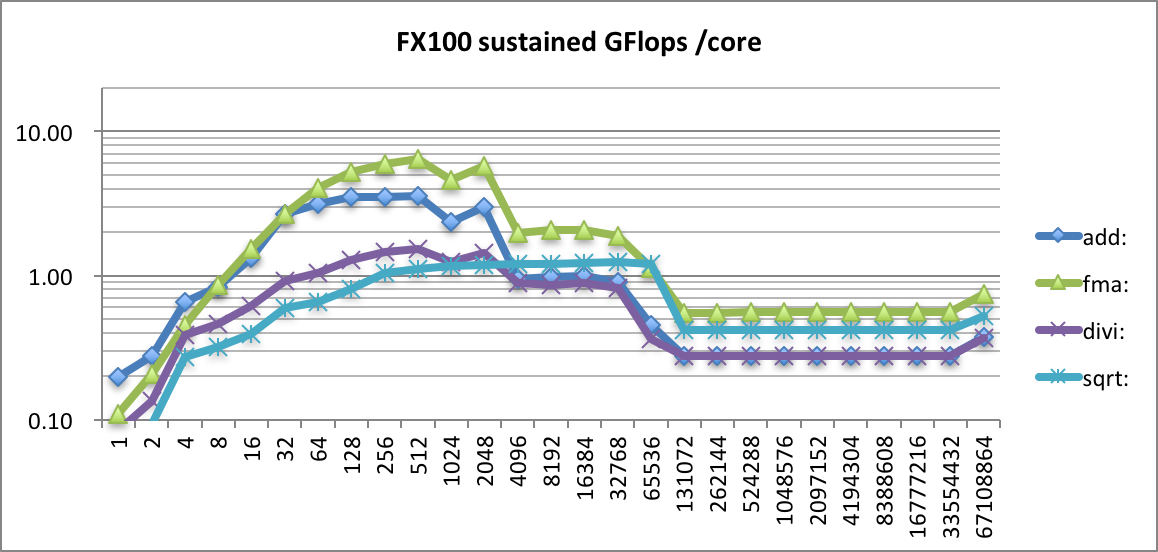
\includegraphics[width=0.45\textwidth]{figs/fx100-gflops-long-R8.pdf}
\caption{fx100-gflops-long-R8}
\label{fig:fx100-gflops-long-R8}
\end{figure}

The displayed curves represent arthmetic performance.
The performance tends to improve according to the increase of
loop length until L1 cache size limit is reached, and drops to
the bandwidth constrained performance level of the next level cash.
This performance tendency matches the reports from other associated research.

In short loop region,
the overhead to process loop set-up and update can not be neglected,
the the performance is bound to data access latency.

In long loop region,
the the performance is bound to
L1\$ / L2\$ / LLC / memory bandwidth in the roofline \cite{Williams:2009}
envelop.

\begin{figure}[tb]
\begin{minipage}{0.48\hsize}
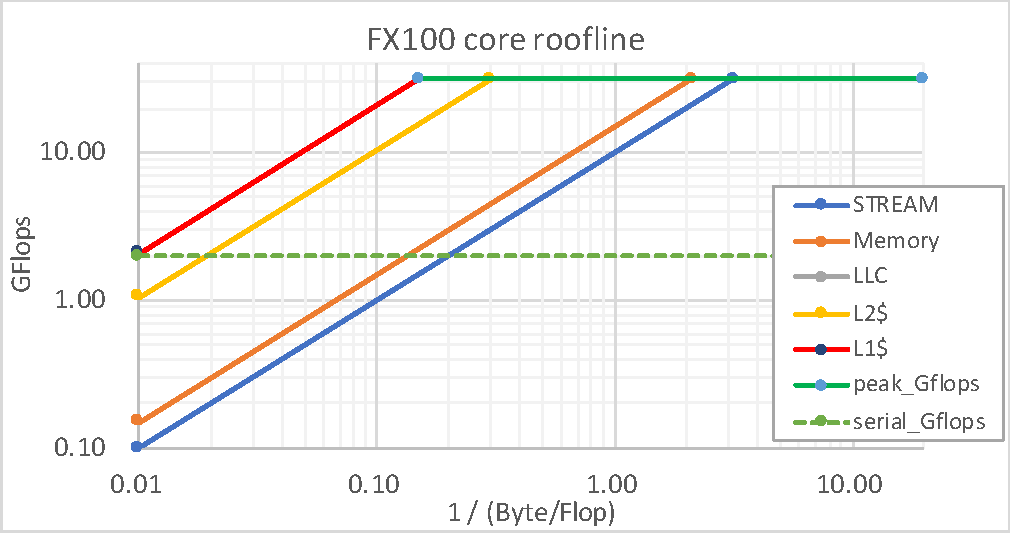
\includegraphics[width=0.98\textwidth]{figs/roofline-fx100.pdf}
\caption{roofline envelop FX100}
\label{fig:roofline-fx100}
\end{minipage}
\begin{minipage}{0.48\hsize}
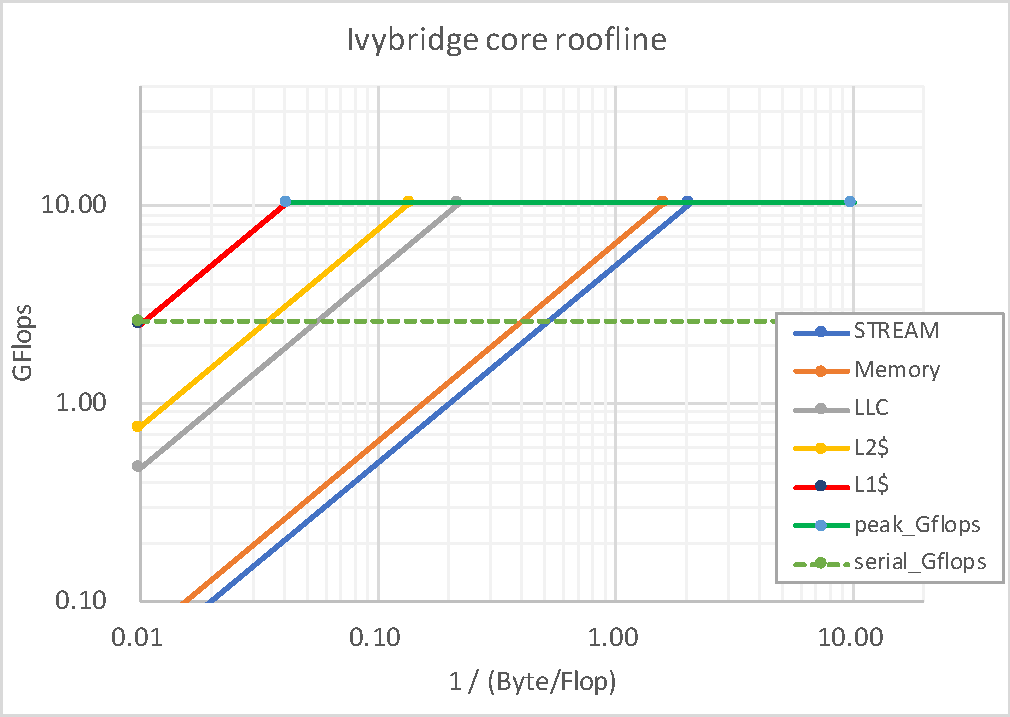
\includegraphics[width=0.98\textwidth]{figs/roofline-ivy.pdf}
\caption{roofline envelop IVY}
\label{fig:roofline-ivy}
\end{minipage}
\end{figure}


Fig.\ref{fig:fx100-gflops-short-R8} and fig.\ref{fig:ivy-gflops-short-R8}
shows the detail performance characteristics of the same kernels for
\begin{math}
n=1,2,3,..,128
\end{math}
and close-up look for
\begin{math}
n=1,2,3,..,50
\end{math}


\begin{figure}[tb]
\centering
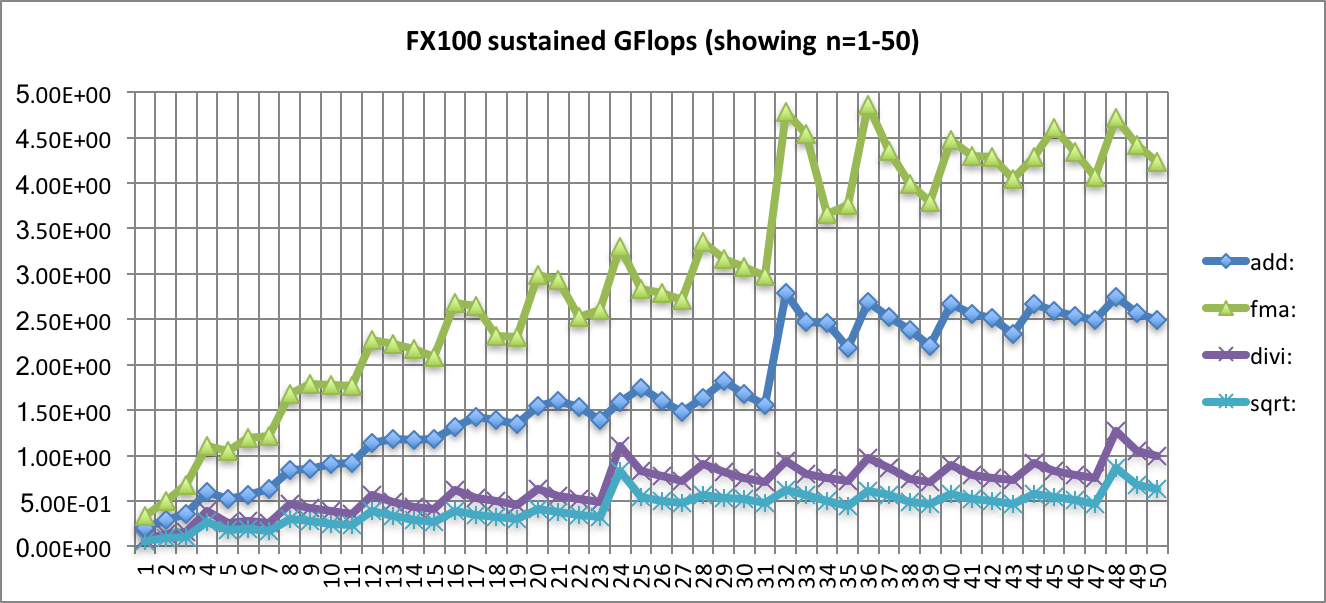
\includegraphics[width=0.45\textwidth]{figs/fx100-gflops-short-R8.pdf}
\caption{fx100-gflops-short-R8}
\label{fig:fx100-gflops-short-R8}
\end{figure}

\begin{figure}[tb]
\centering
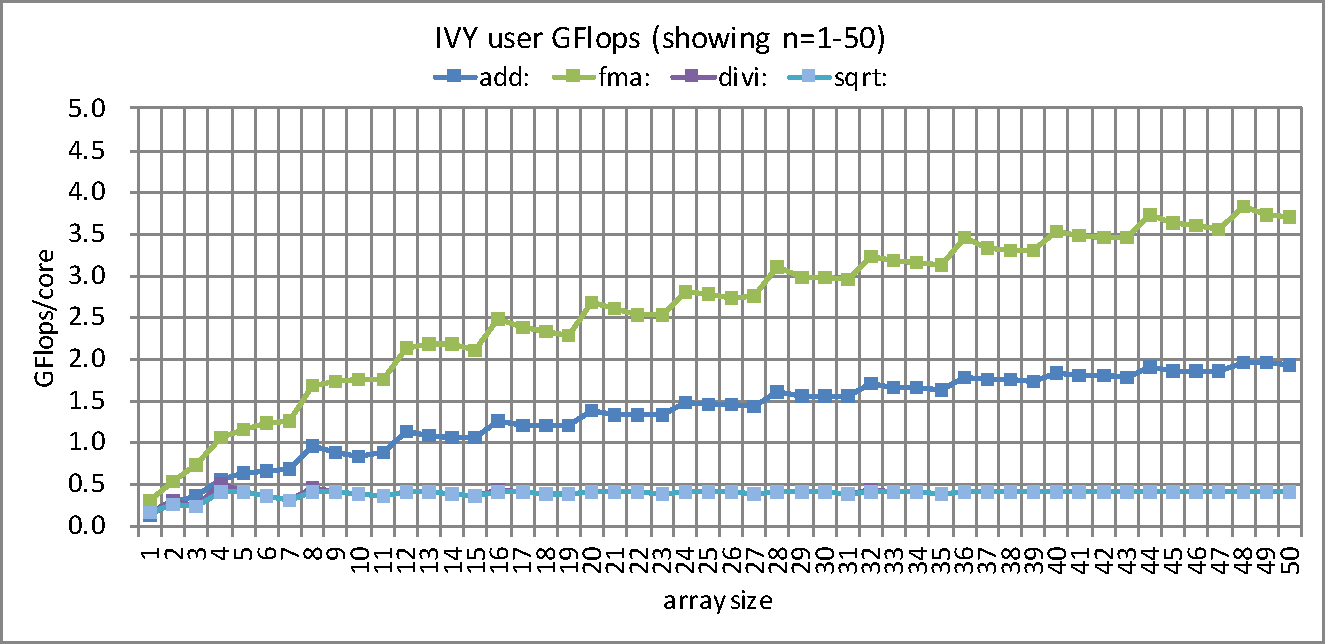
\includegraphics[width=0.45\textwidth]{figs/ivy-gflops-short-R8.pdf}
\caption{ivy-gflops-short-R8}
\label{fig:ivy-gflops-short-R8}
\end{figure}

The detail performance curves does not show gradual increase. Instead, they
show steep stepping shapes at multiple of constant interval.
This is a common observation on systems with SIMD supporting processors,
and the interval corresponds to the data width of SIMD instructions.
For example, FX100 double precision (64 bits) arithmetic can utilize
256 bit instruction, and the resulting interval is
\begin{math}
256 / 64 = 4
\end{math}
.
So the performance is highest at 4n, then 4n+1, 4n+2, and lowest at 4n+3.

The fig.\ref{fig:fx100-gflops-short-R8} is showing the fact that
program coding practice to maintain the loop length as the multiply of
SIMD width has significant impact, especially for short loop computation.

The interval for single precision (32 bits) is
\begin{math}
256 / 32 = 8
\end{math}
, and shows even stronger performance impact as seen in
fig.\ref{fig:fx100-gflops-short-R4} for FX100.

\begin{figure}[tb]
\centering
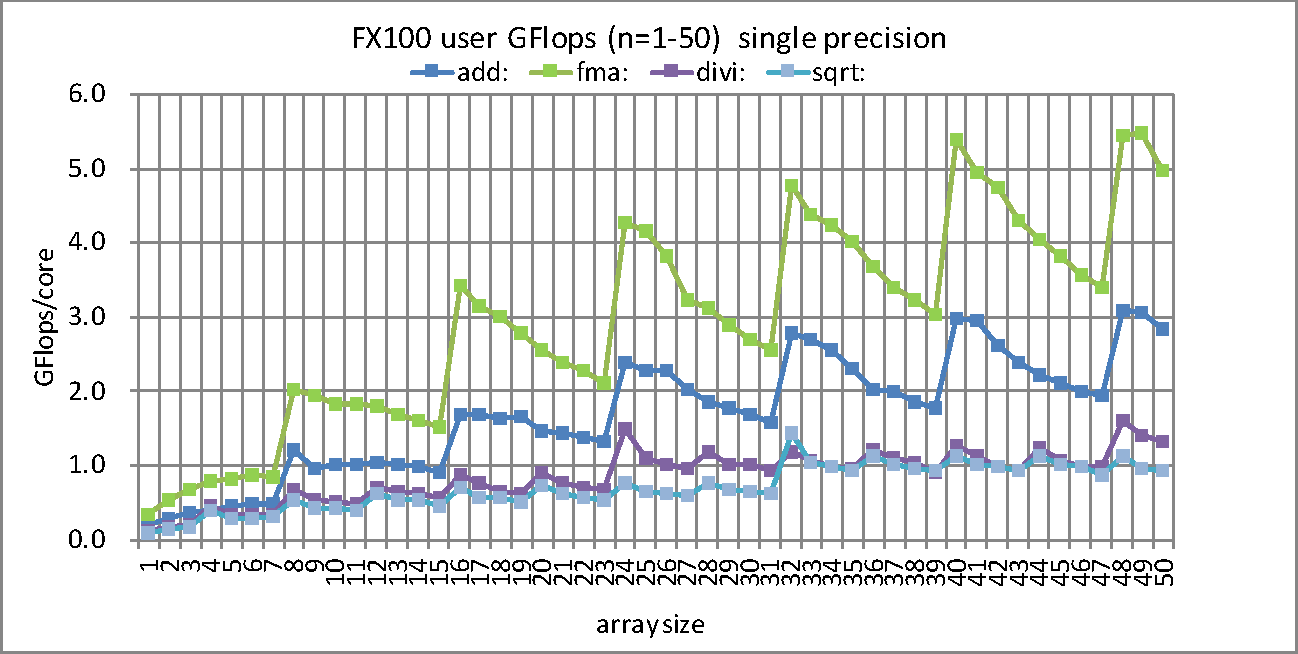
\includegraphics[width=0.45\textwidth]{figs/fx100-gflops-short-R4.pdf}
\caption{fx100-gflops-short-R4}
\label{fig:fx100-gflops-short-R4}
\end{figure}

Performance evaluation from the arithmetic perspective and from the
system perspective provides the capability to build up the theoretical
workload model of the application,
and the capability to map the model with the actual system workload
and performance on a specific HPC system.
PMlib provides the capability to conduct such synthetic performance
evaluation, and hopefully the hint for further optimized execution of
the application in its development and production phase.


\subsection{STREAM}
\label{subsection:STREAM}
STREAM benchmark \cite{stream:1995}
has been widely used to measure the memory bandwidth of the computer systems.
STREAM standard output reports the
basic arithmetic performance of the copy, multiplication, addition,
and multiplication\&addition, i.e. arithmetic workload perspective.

%	As seen in the previous examples {\color{blue}wants ref \ref{} },
STREAM HWPC performance shows different characteristics against
the reported STREAM arithmetic performance. Their performance is under
combined affect of compilers and their optimization options.
Although this paper does not intend to cover those exhaustive combinations,
a few points of interest related to the bandwidth are shown here.
%
The measurement is done on Intel Ivybridge server using Intel 2017 compiler.

The first STREAM Fortran OpenMP result using 8 threads packed in a CPU
is shown in fig.\ref{fig:stream-ivy-1cpux8}.
Then we compare fig.\ref{fig:stream-ivy-1cpux8T}
with
fig.\ref{fig:stream-ivy-4cpux2T} 
which shows the result using 8 threads scattered over 4 CPUs.
%
%	% if without minipage
%	\centering
%	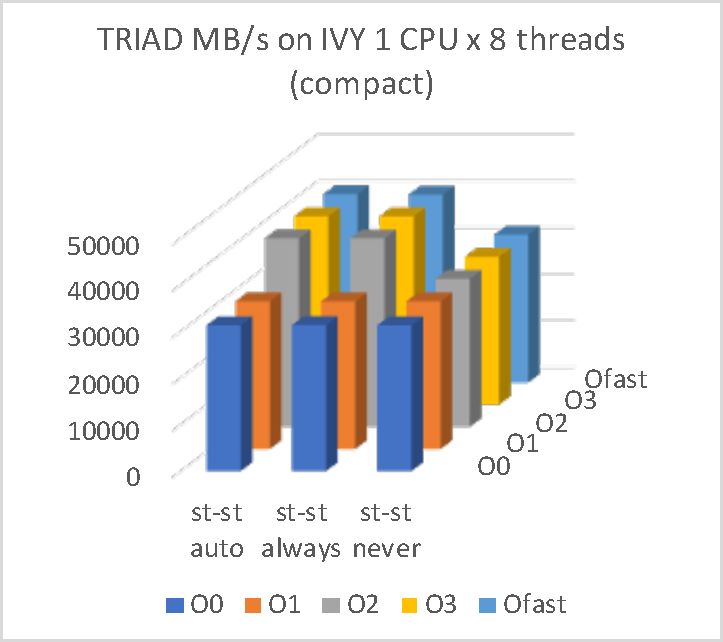
\includegraphics[width=0.45\textwidth]{figs/stream-ivy-1cpux8T.pdf}
%	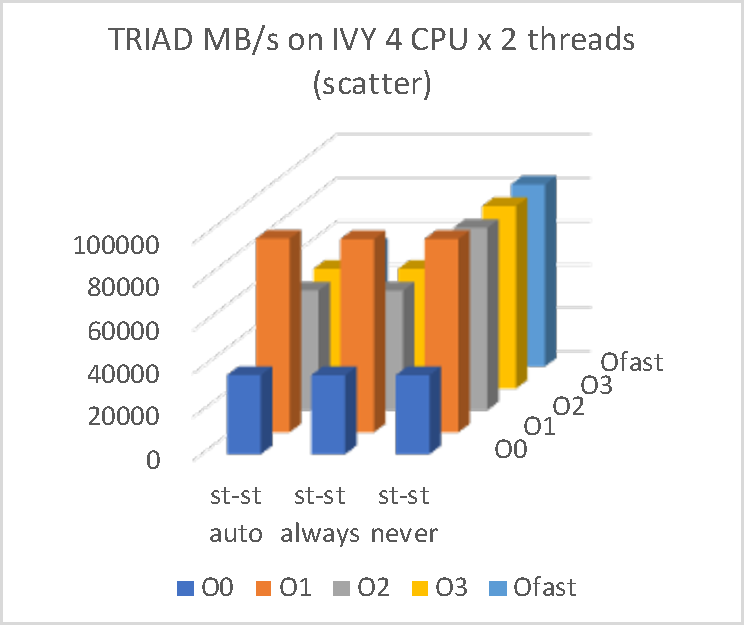
\includegraphics[width=0.45\textwidth]{figs/stream-ivy-4cpux2T.pdf}
%
\begin{figure}[tb]
\begin{minipage}{0.48\hsize}
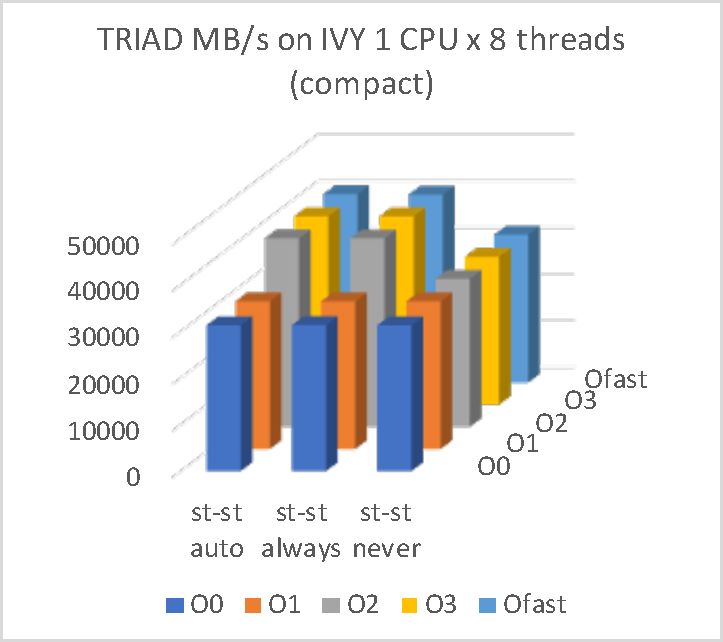
\includegraphics[width=0.98\textwidth]{figs/stream-ivy-1cpux8T.pdf}
\caption{stream-ivy-1cpux8T}
\label{fig:stream-ivy-1cpux8T}
\end{minipage}
\begin{minipage}{0.48\hsize}
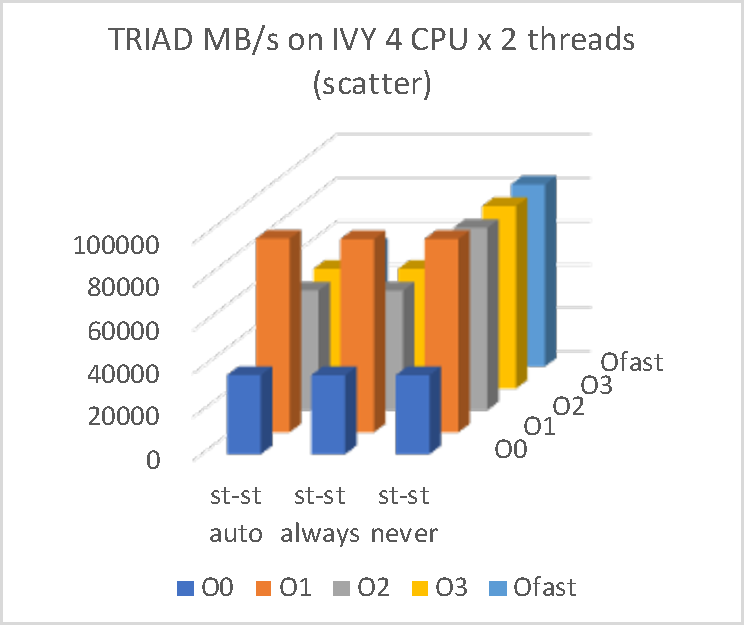
\includegraphics[width=0.98\textwidth]{figs/stream-ivy-4cpux2T.pdf}
\caption{stream-ivy-4cpux2T}
\label{fig:stream-ivy-4cpux2T}
\end{minipage}
\end{figure}


PMlib BANDWIDTH report and CACHE report can be used
to check the data movement in cache and memory layer.
Partial output from the report is shown in listing \ref{tab:report-BANDWIDTH}.

\begin{table*}[tb]
\scriptsize
\caption{PMlib report for BANDWIDTH}
\label{tab:report-BANDWIDTH}
\footnotesize
\begin{tabular}{l} \hline
\scriptsize
\input{figs/stdout.stream-PMlib-BANDWIDTH.txt}
\input{figs/stdout.stream-PMlib-CACHE.txt}
above lines should be long.
add some analysis to above PMlib report for STREAM.
\end{tabular}
\end{table*}


\section{Conclusion}

\section*{Acknowledgment}

\section*{References}

{\color{blue}
citation should be checked before the final submission.\par
Is there good reference/citation for low-performance  or bottleneck-analysis?
}

{\color{blue} Check the use of terminology: user/arithmetic/application/system}

%	\cite{PMlib:webpage-public},
%	\cite{PMlib:webpage-master},
%	\cite{PMlib:webpage-develop},

\bibliographystyle{jplain}
\bibliography{PMlib}
\end{document}

